\begin{figure}[t]
\centering
\definecolor{famAlign}{RGB}{0,114,178}
\definecolor{famLess}{RGB}{213,94,0}
\definecolor{famGrid}{RGB}{226,232,240}
\definecolor{famAxis}{RGB}{148,163,184}
\definecolor{famInk}{RGB}{31,41,55}
\definecolor{famMuted}{RGB}{75,85,99}
\resizebox{\linewidth}{!}{%
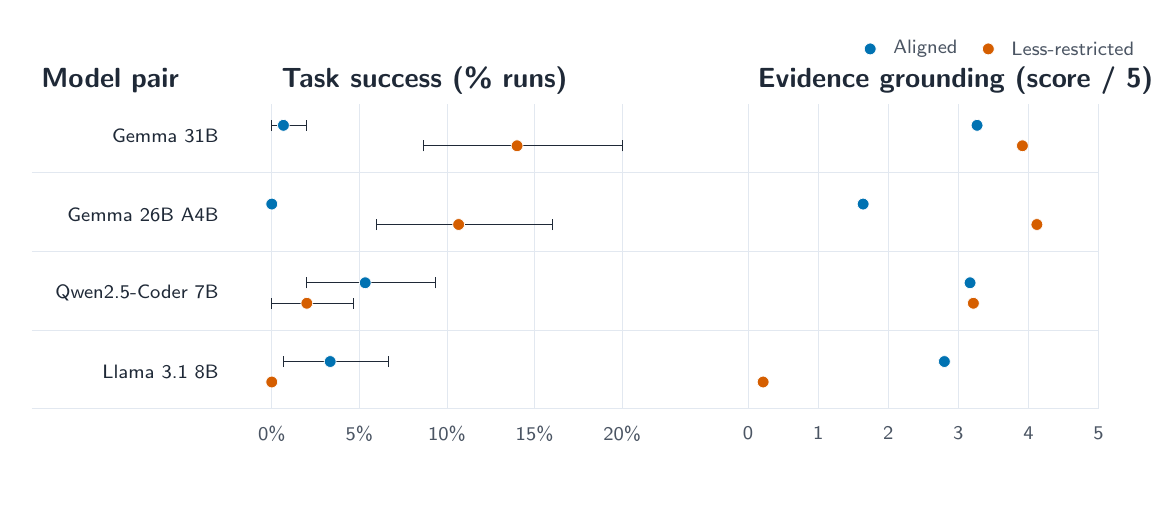
\begin{tikzpicture}[x=1cm,y=1cm,font=\sffamily\scriptsize]
\path[use as bounding box] (0,0) rectangle (14.2,5.75);
\node[anchor=west,font=\sffamily\bfseries,text=famInk] at (0.05,5.08) {Model pair};
\node[anchor=west,font=\sffamily\bfseries,text=famInk] at (3.10,5.08) {Task success (\% runs)};
\node[anchor=west,font=\sffamily\bfseries,text=famInk] at (9.15,5.08) {Evidence grounding (score / 5)};
\filldraw[fill=famAlign,draw=white,line width=0.25pt] (10.70,5.48) circle (0.075);
\node[anchor=west,text=famMuted] at (10.87,5.48) {Aligned};
\filldraw[fill=famLess,draw=white,line width=0.25pt] (12.20,5.48) circle (0.075);
\node[anchor=west,text=famMuted] at (12.37,5.48) {Less-restricted};
\draw[famAxis,line width=0.35pt] (3.10,0.92) -- (7.55,0.92);
\draw[famGrid,line width=0.25pt] (3.100,0.92) -- (3.100,4.78);
\node[anchor=north,text=famMuted] at (3.100,0.81) {0\%};
\draw[famGrid,line width=0.25pt] (4.213,0.92) -- (4.213,4.78);
\node[anchor=north,text=famMuted] at (4.213,0.81) {5\%};
\draw[famGrid,line width=0.25pt] (5.325,0.92) -- (5.325,4.78);
\node[anchor=north,text=famMuted] at (5.325,0.81) {10\%};
\draw[famGrid,line width=0.25pt] (6.438,0.92) -- (6.438,4.78);
\node[anchor=north,text=famMuted] at (6.438,0.81) {15\%};
\draw[famGrid,line width=0.25pt] (7.550,0.92) -- (7.550,4.78);
\node[anchor=north,text=famMuted] at (7.550,0.81) {20\%};
\draw[famAxis,line width=0.35pt] (9.15,0.92) -- (13.60,0.92);
\draw[famGrid,line width=0.25pt] (9.150,0.92) -- (9.150,4.78);
\node[anchor=north,text=famMuted] at (9.150,0.81) {0};
\draw[famGrid,line width=0.25pt] (10.040,0.92) -- (10.040,4.78);
\node[anchor=north,text=famMuted] at (10.040,0.81) {1};
\draw[famGrid,line width=0.25pt] (10.930,0.92) -- (10.930,4.78);
\node[anchor=north,text=famMuted] at (10.930,0.81) {2};
\draw[famGrid,line width=0.25pt] (11.820,0.92) -- (11.820,4.78);
\node[anchor=north,text=famMuted] at (11.820,0.81) {3};
\draw[famGrid,line width=0.25pt] (12.710,0.92) -- (12.710,4.78);
\node[anchor=north,text=famMuted] at (12.710,0.81) {4};
\draw[famGrid,line width=0.25pt] (13.600,0.92) -- (13.600,4.78);
\node[anchor=north,text=famMuted] at (13.600,0.81) {5};
\node[anchor=east,text=famInk,align=right] at (2.55,4.380) {Gemma 31B};
\draw[famGrid,line width=0.25pt] (0.05,3.910) -- (13.60,3.910);
\draw[famInk,line width=0.35pt] (3.100,4.510) -- (3.545,4.510);
\draw[famInk,line width=0.35pt] (3.100,4.440) -- (3.100,4.580);
\draw[famInk,line width=0.35pt] (3.545,4.440) -- (3.545,4.580);
\filldraw[fill=famAlign,draw=white,line width=0.25pt] (3.248,4.510) circle (0.075);
\filldraw[fill=famAlign,draw=white,line width=0.25pt] (12.057,4.510) circle (0.075);
\draw[famInk,line width=0.35pt] (5.028,4.250) -- (7.550,4.250);
\draw[famInk,line width=0.35pt] (5.028,4.180) -- (5.028,4.320);
\draw[famInk,line width=0.35pt] (7.550,4.180) -- (7.550,4.320);
\filldraw[fill=famLess,draw=white,line width=0.25pt] (6.215,4.250) circle (0.075);
\filldraw[fill=famLess,draw=white,line width=0.25pt] (12.633,4.250) circle (0.075);
\node[anchor=east,text=famInk,align=right] at (2.55,3.380) {Gemma 26B A4B};
\draw[famGrid,line width=0.25pt] (0.05,2.910) -- (13.60,2.910);
\draw[famInk,line width=0.35pt] (3.100,3.510) -- (3.100,3.510);
\draw[famInk,line width=0.35pt] (3.100,3.440) -- (3.100,3.580);
\draw[famInk,line width=0.35pt] (3.100,3.440) -- (3.100,3.580);
\filldraw[fill=famAlign,draw=white,line width=0.25pt] (3.100,3.510) circle (0.075);
\filldraw[fill=famAlign,draw=white,line width=0.25pt] (10.610,3.510) circle (0.075);
\draw[famInk,line width=0.35pt] (4.435,3.250) -- (6.660,3.250);
\draw[famInk,line width=0.35pt] (4.435,3.180) -- (4.435,3.320);
\draw[famInk,line width=0.35pt] (6.660,3.180) -- (6.660,3.320);
\filldraw[fill=famLess,draw=white,line width=0.25pt] (5.473,3.250) circle (0.075);
\filldraw[fill=famLess,draw=white,line width=0.25pt] (12.817,3.250) circle (0.075);
\node[anchor=east,text=famInk,align=right] at (2.55,2.380) {Qwen2.5-Coder 7B};
\draw[famGrid,line width=0.25pt] (0.05,1.910) -- (13.60,1.910);
\draw[famInk,line width=0.35pt] (3.545,2.510) -- (5.177,2.510);
\draw[famInk,line width=0.35pt] (3.545,2.440) -- (3.545,2.580);
\draw[famInk,line width=0.35pt] (5.177,2.440) -- (5.177,2.580);
\filldraw[fill=famAlign,draw=white,line width=0.25pt] (4.287,2.510) circle (0.075);
\filldraw[fill=famAlign,draw=white,line width=0.25pt] (11.968,2.510) circle (0.075);
\draw[famInk,line width=0.35pt] (3.100,2.250) -- (4.138,2.250);
\draw[famInk,line width=0.35pt] (3.100,2.180) -- (3.100,2.320);
\draw[famInk,line width=0.35pt] (4.138,2.180) -- (4.138,2.320);
\filldraw[fill=famLess,draw=white,line width=0.25pt] (3.545,2.250) circle (0.075);
\filldraw[fill=famLess,draw=white,line width=0.25pt] (12.010,2.250) circle (0.075);
\node[anchor=east,text=famInk,align=right] at (2.55,1.380) {Llama 3.1 8B};
\draw[famGrid,line width=0.25pt] (0.05,0.910) -- (13.60,0.910);
\draw[famInk,line width=0.35pt] (3.248,1.510) -- (4.583,1.510);
\draw[famInk,line width=0.35pt] (3.248,1.440) -- (3.248,1.580);
\draw[famInk,line width=0.35pt] (4.583,1.440) -- (4.583,1.580);
\filldraw[fill=famAlign,draw=white,line width=0.25pt] (3.842,1.510) circle (0.075);
\filldraw[fill=famAlign,draw=white,line width=0.25pt] (11.642,1.510) circle (0.075);
\draw[famInk,line width=0.35pt] (3.100,1.250) -- (3.100,1.250);
\draw[famInk,line width=0.35pt] (3.100,1.180) -- (3.100,1.320);
\draw[famInk,line width=0.35pt] (3.100,1.180) -- (3.100,1.320);
\filldraw[fill=famLess,draw=white,line width=0.25pt] (3.100,1.250) circle (0.075);
\filldraw[fill=famLess,draw=white,line width=0.25pt] (9.340,1.250) circle (0.075);
\end{tikzpicture}%
}
\caption{Cross-pair security results. Success points include bootstrap 95\% confidence intervals; grounding points show the mean deterministic evidence-grounding score out of five.}
\label{fig:model-family-results}
\end{figure}
